\documentclass[a4paper,11pt]{article}

\usepackage[T1]{fontenc}

\usepackage[utf8]{inputenc}

\usepackage[italian]{babel}

\usepackage{graphicx}

\usepackage{indentfirst}

\usepackage{amsmath,amssymb}

\usepackage{enumitem} 

\newcommand{\virgolette}[1]{``#1''}

\usepackage[margin=1in]{geometry} %Smaller margins

\usepackage{lmodern} %Vector PDF

\usepackage{siunitx}

\usepackage{xcolor}

\usepackage{colortbl}

\usepackage{booktabs}

\usepackage{graphicx}
\graphicspath{ {../Immagini/} }

\usepackage{wrapfig}

\usepackage{siunitx} % Per unit� di misura in generale e la corretta rappresentazione dei numeri.

\begin{document}

\begin{titlepage}
	\centering
	{\scshape\LARGE Laboratorio di Ottica, Elettronica e \\ Fisica Moderna \par}
	\vspace{1cm}
	{\scshape\Large Relazione di Laboratorio 5\par}
	\vspace{1.5cm}
	{\huge\bfseries Rapporto carica massa dell'elettrone\par}
	\vspace{2cm}

	{\Large\itshape Nicolò Cavalleri, Giacomo Lini e Davide Passaro
		
	(LUN12)}

	\vspace{5cm}
	\vfill

	\begin{abstract}
		Questo documento contiene la procedura e l'analisi dati di un esperimento volto a misurare il rapporto tra la carica e la massa dell'elettrone. L'esperimento seguito non corrisponde a quello di Thompson (il primo esperimento che ottenne questa misura) ma una variante che, utilizzando una coppia di bobine di Helmholtz, riesce a produrre un campo magnetico più facilmente misurabile.
	\end{abstract}


	\vfill
	{\large \today\par}
	
\end{titlepage}

\newpage

	\section{Introduzione}
	\begin{wrapfigure}{r}{0.5\textwidth}
		\centering
		\vspace{-0.5cm}
		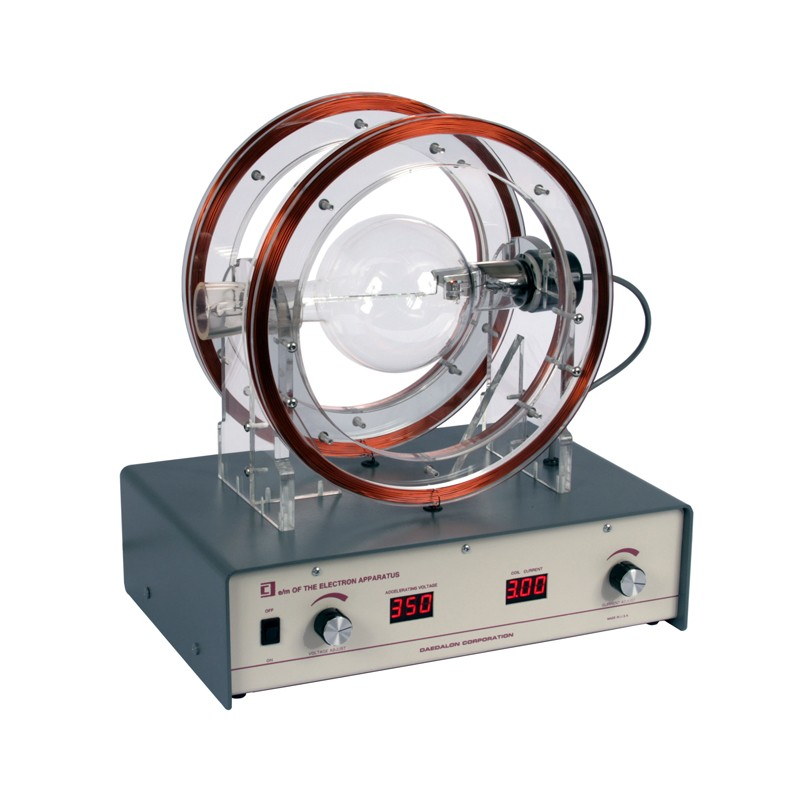
\includegraphics[width=0.5\textwidth]{apparatus}
		
		\label{apparato}
		\caption{Fotografia di un apparato simile a quello utilizzato nell'esperimento}
	\end{wrapfigure}
	L'esperimento si propone di misurare il rapporto tra la massa e la carica dell'elettrone. Questo esperimento, è stato (nella variante di J. J. Thompson) rivoluzionario per la fisica in quanto ha segnato l'inizio dello studio delle particelle fondamentali e in generale della fisica subatomica. Infatti questo esperimento provò definitivamente l'esistenza di particelle cariche negativamente (elettroni) che costituivano un argomento molto discusso e controverso anche tra i più grandi fisici dell'Ottocento. Controversie che, poco dopo, con la misura della carica dell'elettrone furono completamente risolte con la realizzazione che queste particelle avessero massa molto più piccola di quella dell'atomo di idrogeno, storicamente considerato la \virgolette{particella} più leggera esistente.
	
	In breve il procedimento seguito si è basato sulla misura della traiettoria di un fascio di elettroni sotto l'effetto di un campo elettrico ed uno magnetico. Il primo è servito per accelerare gli elettroni mentre il secondo è servito per deviare a traiettoria in un moto rettilineo uniforme di cui abbiamo facilmente calcolato il raggio.
	
	Per produrre il campo elettrico è stato utilizzato un cannone elettronico mentre per produrre il campo magnetico è stato utilizzato un sistema costituito da bobine di Helmholtz. Attraverso questi strumenti, descritti poi in seguito, siamo riusciti a creare dei campi facilmente misurabili e a modularli secondo le nostre esigenze.
	
	Infine grazie ad un'ampolla tenuta a pressione molto bassa contenente idrogeno siamo riusciti a vedere ad occhio nudo il fascio di elettroni e quindi a calcolare il raggio. 
	
	Sempre attraverso un sistema costituito da bobine di Helmholtz siamo riusciti a misurare la componente tangenziale al terreno del campo magnetico terrestre. Tutte le misure effettuate si sono rilevate compatibili con le aspettative, e nonostante molti problemi pratici descritti in seguito siamo riusciti ad ottenere delle misure abbastanza precise.
	
		\section{Strumentazione}
		
		Qui di seguito sono elencati i pezzi dell'apparato sperimentale usato per portare a termine l'esperimento.
		\begin{description}[align=left]
			
			\item [Ampolla di vetro] usata come ambiente dell'esperimento. L'ampolla, di diametro misurato, conteneva gas idrogeno alla pressione di circa $\SI{E-2}{torr}$, necessario per visualizzare il fascio di elettroni, che, in virtù dell'energia acquistata, ne eccitano gli atomi. Il decadimento sullo stato fondamentale avviene rapidamente ed emette una lunghezza d'onda nella regione tra l'azzurro e il violetto.
			
			\item [Due elettrodi] utilizzati per generare la differenza di potenziale necessaria ad accelerare gli elettroni. L'anodo di forma sommariamente conica è forato per permettere il passaggio degli elettroni ed è sagomato in modo tale da formare un fascio di elettroni ben collimato. Il catodo è riscaldato da un \textbf{filamento} percorso da corrente e gli elettroni sono emessi da quest'ultimo per effetto termoelettronico.
			
			\item [Due bobine di Helmholtz] attraverso cui passa una corrente di intensità $I$, che produce un campo di induzione magnetica $B _z$. La configurazione delle bobine è tale da produrre un campo altamente uniforme nella regione centrale. Il raggio medio e il numero di spire sono forniti dal costruttore.
			
			\item [Specchio] usato per misurare il diametro del fascio di elettroni. Guardando il fascio in modo tale da sovrapporlo alla sua immagine nello specchio si evita infatti l'errore di parallasse.
			
			\item [Un voltametro] usato per misurare la differenza di potenziale usata per accelerare gli elettroni.
			
			\item [Un amperometro] usato per misurare la corrente delle bobine. In particolare è un tester a 3 cifre.
			
			\item [Opportuni trasformatori] utilizzati per regolare le correnti presenti nell'esperimento. Il generatore della tensione anodica non poteva superare i $\SI{300}{V}$.
			
			\item [Calibro elettronico] utilizzato per misurare il fascio di elettroni, opportunamente puntato con un mirino.
			
			\item[Metro] Utilizzato per misurare le grandezze in gioco, men che il diametro del fascio.
			
			\item [Un apparato sperimentale] già costruito composto da due bobine ed una bussola, necessario per misurare la componente orizzontale del campo magnetico terrestre.
			
			Ovviamente era presente anche un supporto su cui era montato l'intero apparato, la cui forma tuttavia non dovrebbe inficiare minimamente sul risultato dell'esperimento.
			
		\end{description}
		
		
		\section{Procedura sperimentale}
		
		Come prima cosa si è costruito il circuito necessario a far passare una corrente dai parametri conosciuti nelle bobine ed una corrente nel filamento all'interno del cannone di elettroni. La modalità di costruzione del circuito era indicata sul supporto per cui assumiamo una corretta impostazione. Una volta accesi tutti i trasformatori, il voltametro e l'amperometro ci si è portati a una condizione tale da vedere il fascio di elettroni, e si è regolato opportunamente la corrente nelle bobine in modo da far compiere agli elettroni un moto circolare uniforme. Ruotando tutto l'apparato si è potuta dedurre la direzione del campo magnetico terrestre, infatti il diametro del fascio di elettroni era minimo quando il campo terrestre era parallelo ed equiorientato al campo generato dalle bobine e massimo quando questo era parallelo ma orientato in senso opposto. Con questa informazione si poteva ruotare l'apparato in modo tale da avere il campo magnetico delle bobine perpendicolare a quello terrestre. Una volta verificato il corretto funzionamento dell'apparato abbiamo cominciato a prendere le misure.
		
		Per ogni misura come prima cosa si regolava la differenza di potenziale applicata al cannone di elettroni. Sono state fatte una dozzina di misure nel range $180 V - 300 V$: sotto i $180 V$ il fascio era poco visibile e per via dei limiti dell'apparato non si potevano superare i $300 V$. Una volta ottenuta la differenza di potenziale desiderata si regolava l'intensità del campo magnetico modificando l'intensità di corrente passante nelle bobine in modo tale da avere un diametro del fascio approssimativamente pari al doppio della distanza del cannone dal centro delle bobine. In questo modo gli elettroni descrivevano una circonferenza con centro sulla retta passante per i centri delle due bobine e l'approssimazione di campo magnetico uniforme era maggiormente soddisfatta. A questo punto si misurava il diametro del fascio, misura con errore maggiore, evitando l'errore di parallasse grazie all'aiuto di uno specchio. Come già accennato si guardava il fascio in modo tale che esso si sovrapponesse alla sua immagine nello specchio e che si sovrapponesse ad entrambi anche il traguardo mobile su cui poi veniva fatta la misura.
		
		Dopo la procedura illustrata si era in possesso di tutte le informazioni necessarie per calcolare il rapporto $e / m $. Infatti, trascurando l'energia cinetica iniziale si ha, per conservazione dell'energia, l'equazione $$ \frac{mv^2}{2} = e \Delta V.$$ Il campo magnetico generato dalle bobine sul loro asse vale invece $$ B _z (0) = \mu _0 \frac{8}{5 \sqrt{5}} \cdot \frac{NI}{R_b}$$ dove $N$ è il numero di spire e $R_b$ il suo raggio medio. A meno di un leggero fattore di correzione, considerando il campo magnetico uniforme in tutta l'ampolla pari al campo magnetico presente sull'asse delle bobine si ha che la forza centripeta vale $$\frac{m v^2}{R} = evB_z$$ e, mettendo quest'equazione a sistema con quella della conservazione dell'energia, si ricava $$\frac{e}{m} = \frac{2 \Delta V}{(B _z R)^2}$$ che è la misura desiderata. Per avere una stima migliore del rapporto, come si vedrà in analisi dati, si utilizza questa equazione per una regressione lineare. Come anticipato si può ricavare per via teorica un fattore di correzione del campo magnetico, per ovviare alla sua non uniformità. I valori del fattore di correzione saranno riportati nella sezione dell'analisi dati.
		
		Una volta ottenuto un numero di misure sufficienti ed aver verificato che abbiano senso, si ripete l'intera procedura orientando l'asse delle bobine parallelamente al campo magnetico terrestre.
		
		Si passa poi alla fase finale dell'esperimento, ossia alla misurazione della componente orizzontale del campo terrestre. Per fare questo si orienta un ago magnetico parallelamente a quest'ultimo e si genera, con delle bobine di raggio e corrente nota un campo magnetico perpendicolare. È intuitivo che maggiore sia la componente orizzontale terrestre maggiore debba essere l'intensità del campo magnetico artificiale per deviare l'ago. La corrente che giunge alle bobine passa attraverso una resistenza che permette una regolazione più fine della corrente entrante. Si misura quindi la corrente necessaria a deflettere l'ago di un angolo $\theta$ e, invertendo la corrente si verifica che l'angolo diventi $-	\theta$. A questo punto il valore della misura si ricava facilmente dall'equazione $$\frac{B_z}{B_t - B_r} = \tan \theta$$ dove $B_t$ è la componente del campo magnetico terrestre mentre $B _z$ e $B_ r$ le componenti del campo magnetico generato dalle bobine, calcolate a partire da un'intensità di corrente pari a $I _0 = \SI{100}{\milli A}$.
		
		\section{Raccolta e Analisi Dati}
		
		La procedura di raccolta e di analisi dei dati per il calcolo del rapporto $e/m$ consiste principalmente nella registrazione del valore del raggio della circonferenza del fascio di elettroni \virgolette{sparato} per diversi valori di corrente e differenti differenza di potenziale. In questo modo per variazioni del campo magnetico prodotto dalle bobine di Helmholtz e del potenziale applicato al catodo che emette gli elettroni è possbile verificare la relazione lineare:
		\begin{equation}\label{regressione}
		(B_z R)^2 = 2\Delta V \, m/e 
		\end{equation}
		dove $\Delta V$ è la differenza di potenziale applicata, $B_z$ è il capo magnetico prodotto dalle bobine di Helmholtz in funzione della corrente. Invertendo questa relazione è possibile individuare il valore di $e/m$. Questo calcolo viene fatto in due condizioni sperimentali differenti: in condizione di perpendicolarità tra campo magnetico terrestre e campo prodotto dalle bobine, e in condizione di anti-parallelismo.
		
		A queste procedure sperimentali è stata affiancata una seconda fase sperimentale in cui sono state effettuate diverse misure dell'intensità del campo magnetico terrestre $B_t$, ricavato dalla relazione:
		\begin{equation}\label{B_terra}
		B_t= \frac{I}{I_0} (B_z \cot \theta + B_r) 
		\end{equation}
		dove $B_z$ e $B_r$ sono le componenti del campo magnetico generato dalle bobine dell'apparato di misura, e $\theta$ è l'angolo misurato sul goniometro
		Questi dati sono necessari per una corretta valutazione dell'intensità del campo generato dalle bobine in situazione di antiparallelismo. La presenza del campo magnetico terrestre ha infatti una influenza apprezzabile sul campo generato dalle bobine, e non può essere trascurato. Terremo la separazione tra misura del rapporto $e/m$ e misura del campo magnetico terrestre.
		
		\subsection{Raccolta Dati - Misura del rapporto $e/m$}
		
		La raccolta di dati consiste come descritto precedentemente nella regisrazione del raggio della circonferenza descritta dal fascio di elettroni deviati dal campo magnetico. In considerazione del fatto che risulta piuttoso difficile riuscire a far collimare i fermi con la posizione del raggio, anche servendosi dello specchio, si è deciso di prendere come errore per la misura del raggio $\sigma_R = \SI{5}{\milli\meter}$, valore che corrisponde a un errore percentuale dell'oridine del $4-5\%$ a seconda del raggio misurato. Di seguito le tabelle \ref{dati_perpendicolare} e \ref{dati_parallelo} riportano i valori ottenuti dei raggi, delle differenze di tensione, delle correnti applicate, e del campo magnetico\footnote{Ai valori del campo magnetico è già stato applicato il fattore di correzione opportuno}, con gli errori annessi su campioni di 11-13 misurazioni\footnote{Per quanto riguarda la tabella \ref{dati_parallelo}, i valori di raggio da una certa misurazione sono uguali. Questo perchè, senza perdita di precisione nella misura, si è scelto di lasciare fermi i perni dell'asta attaccata all'ampolla, e di modificare i valori di corrente e tensione fino a centrare la posizione dei fermi stessi da cui poi è stata efettuata la lettura. In questo modo si sono sveltite le procedure di misurazione senza perdita di generalità della procedura, come mostrato dai dati raccolti.}.
		
		
		% Please add the following required packages to your document preamble:
		% \usepackage[table,xcdraw]{xcolor}
		% If you use beamer only pass "xcolor=table" option, i.e. \documentclass[xcolor=table]{beamer}
		\begin{table}[]
			\centering
			\caption{Dati misura $e/m$ - perpendicolare}
			\label{dati_perpendicolare}
			\begin{tabular}{lrrrrrrrr}
				\rowcolor[HTML]{BBDAFF} 
				\multicolumn{1}{c}{\cellcolor[HTML]{BBDAFF}}    & \multicolumn{1}{l}{\cellcolor[HTML]{BBDAFF}$R (\SI{}{\meter})$} & $\sigma_R  $                                         & \multicolumn{1}{l}{\cellcolor[HTML]{BBDAFF}$\Delta V (\SI{}{\volt})$} & \multicolumn{1}{l}{\cellcolor[HTML]{BBDAFF}$\sigma_V$} & \multicolumn{1}{l}{\cellcolor[HTML]{BBDAFF}$I (\SI{}{\ampere}$)} & \multicolumn{1}{l}{\cellcolor[HTML]{BBDAFF}$\sigma_I$} & \multicolumn{1}{l}{\cellcolor[HTML]{BBDAFF}$B_z(R) (\SI{}{\tesla})$} & \multicolumn{1}{l}{\cellcolor[HTML]{BBDAFF}$\sigma_B$} \\ \cline{2-9} 
				\rowcolor[HTML]{C0C0C0} 
				\multicolumn{1}{l|}{\cellcolor[HTML]{BBDAFF}1}  & \multicolumn{1}{r|}{\cellcolor[HTML]{C0C0C0}0.05352}              & \multicolumn{1}{r|}{\cellcolor[HTML]{C0C0C0}0.0050} & \multicolumn{1}{r|}{\cellcolor[HTML]{C0C0C0}229.2}                        & \multicolumn{1}{r|}{\cellcolor[HTML]{C0C0C0}3.0}       & \multicolumn{1}{r|}{\cellcolor[HTML]{C0C0C0}1.229}               & \multicolumn{1}{r|}{\cellcolor[HTML]{C0C0C0}0.020}     & \multicolumn{1}{r|}{\cellcolor[HTML]{C0C0C0}9.0545E-04}                  & \multicolumn{1}{r|}{\cellcolor[HTML]{C0C0C0}5.55E-06}  \\ \cline{2-9} 
				\rowcolor[HTML]{EFEFEF} 
				\multicolumn{1}{l|}{\cellcolor[HTML]{BBDAFF}2}  & \multicolumn{1}{r|}{\cellcolor[HTML]{EFEFEF}0.05563}              & \multicolumn{1}{r|}{\cellcolor[HTML]{EFEFEF}0.0050} & \multicolumn{1}{r|}{\cellcolor[HTML]{EFEFEF}210.5}                        & \multicolumn{1}{r|}{\cellcolor[HTML]{EFEFEF}3.0}       & \multicolumn{1}{r|}{\cellcolor[HTML]{EFEFEF}1.102}               & \multicolumn{1}{r|}{\cellcolor[HTML]{EFEFEF}0.020}     & \multicolumn{1}{r|}{\cellcolor[HTML]{EFEFEF}8.1140E-04}                  & \multicolumn{1}{r|}{\cellcolor[HTML]{EFEFEF}4.97E-06}  \\ \cline{2-9} 
				\rowcolor[HTML]{C0C0C0} 
				\multicolumn{1}{l|}{\cellcolor[HTML]{BBDAFF}3}  & \multicolumn{1}{r|}{\cellcolor[HTML]{C0C0C0}0.05276}              & \multicolumn{1}{r|}{\cellcolor[HTML]{C0C0C0}0.0050} & \multicolumn{1}{r|}{\cellcolor[HTML]{C0C0C0}243.3}                        & \multicolumn{1}{r|}{\cellcolor[HTML]{C0C0C0}3.0}       & \multicolumn{1}{r|}{\cellcolor[HTML]{C0C0C0}1.204}               & \multicolumn{1}{r|}{\cellcolor[HTML]{C0C0C0}0.020}     & \multicolumn{1}{r|}{\cellcolor[HTML]{C0C0C0}8.8796E-04}                  & \multicolumn{1}{r|}{\cellcolor[HTML]{C0C0C0}5.44E-06}  \\ \cline{2-9} 
				\rowcolor[HTML]{EFEFEF} 
				\multicolumn{1}{l|}{\cellcolor[HTML]{BBDAFF}4}  & \multicolumn{1}{r|}{\cellcolor[HTML]{EFEFEF}0.05125}              & \multicolumn{1}{r|}{\cellcolor[HTML]{EFEFEF}0.0050} & \multicolumn{1}{r|}{\cellcolor[HTML]{EFEFEF}277.3}                        & \multicolumn{1}{r|}{\cellcolor[HTML]{EFEFEF}3.0}       & \multicolumn{1}{r|}{\cellcolor[HTML]{EFEFEF}1.389}               & \multicolumn{1}{r|}{\cellcolor[HTML]{EFEFEF}0.020}     & \multicolumn{1}{r|}{\cellcolor[HTML]{EFEFEF}1.0244E-03}                  & \multicolumn{1}{r|}{\cellcolor[HTML]{EFEFEF}6.28E-06}  \\ \cline{2-9} 
				\rowcolor[HTML]{C0C0C0} 
				\multicolumn{1}{l|}{\cellcolor[HTML]{BBDAFF}5}  & \multicolumn{1}{r|}{\cellcolor[HTML]{C0C0C0}0.05468}              & \multicolumn{1}{r|}{\cellcolor[HTML]{C0C0C0}0.0050} & \multicolumn{1}{r|}{\cellcolor[HTML]{C0C0C0}281.7}                        & \multicolumn{1}{r|}{\cellcolor[HTML]{C0C0C0}3.0}       & \multicolumn{1}{r|}{\cellcolor[HTML]{C0C0C0}1.333}               & \multicolumn{1}{r|}{\cellcolor[HTML]{C0C0C0}0.020}     & \multicolumn{1}{r|}{\cellcolor[HTML]{C0C0C0}9.8149E-04}                  & \multicolumn{1}{r|}{\cellcolor[HTML]{C0C0C0}6.01E-06}  \\ \cline{2-9} 
				\rowcolor[HTML]{EFEFEF} 
				\multicolumn{1}{l|}{\cellcolor[HTML]{BBDAFF}6}  & \multicolumn{1}{r|}{\cellcolor[HTML]{EFEFEF}0.05175}              & \multicolumn{1}{r|}{\cellcolor[HTML]{EFEFEF}0.0050} & \multicolumn{1}{r|}{\cellcolor[HTML]{EFEFEF}296.2}                        & \multicolumn{1}{r|}{\cellcolor[HTML]{EFEFEF}3.0}       & \multicolumn{1}{r|}{\cellcolor[HTML]{EFEFEF}1.450}               & \multicolumn{1}{r|}{\cellcolor[HTML]{EFEFEF}0.020}     & \multicolumn{1}{r|}{\cellcolor[HTML]{EFEFEF}1.0694E-03}                  & \multicolumn{1}{r|}{\cellcolor[HTML]{EFEFEF}6.55E-06}  \\ \cline{2-9} 
				\rowcolor[HTML]{C0C0C0} 
				\multicolumn{1}{l|}{\cellcolor[HTML]{BBDAFF}7}  & \multicolumn{1}{r|}{\cellcolor[HTML]{C0C0C0}0.05612}              & \multicolumn{1}{r|}{\cellcolor[HTML]{C0C0C0}0.0050} & \multicolumn{1}{r|}{\cellcolor[HTML]{C0C0C0}184}                          & \multicolumn{1}{r|}{\cellcolor[HTML]{C0C0C0}3.0}       & \multicolumn{1}{r|}{\cellcolor[HTML]{C0C0C0}1.000}               & \multicolumn{1}{r|}{\cellcolor[HTML]{C0C0C0}0.020}     & \multicolumn{1}{r|}{\cellcolor[HTML]{C0C0C0}7.3586E-04}                  & \multicolumn{1}{r|}{\cellcolor[HTML]{C0C0C0}4.51E-06}  \\ \cline{2-9} 
				\rowcolor[HTML]{EFEFEF} 
				\multicolumn{1}{l|}{\cellcolor[HTML]{BBDAFF}8}  & \multicolumn{1}{r|}{\cellcolor[HTML]{EFEFEF}0.05984}              & \multicolumn{1}{r|}{\cellcolor[HTML]{EFEFEF}0.0050} & \multicolumn{1}{r|}{\cellcolor[HTML]{EFEFEF}199.6}                        & \multicolumn{1}{r|}{\cellcolor[HTML]{EFEFEF}3.0}       & \multicolumn{1}{r|}{\cellcolor[HTML]{EFEFEF}1.019}               & \multicolumn{1}{r|}{\cellcolor[HTML]{EFEFEF}0.020}     & \multicolumn{1}{r|}{\cellcolor[HTML]{EFEFEF}7.4773E-04}                  & \multicolumn{1}{r|}{\cellcolor[HTML]{EFEFEF}4.58E-06}  \\ \cline{2-9} 
				\rowcolor[HTML]{C0C0C0} 
				\multicolumn{1}{l|}{\cellcolor[HTML]{BBDAFF}9}  & \multicolumn{1}{r|}{\cellcolor[HTML]{C0C0C0}0.05277}              & \multicolumn{1}{r|}{\cellcolor[HTML]{C0C0C0}0.0050} & \multicolumn{1}{r|}{\cellcolor[HTML]{C0C0C0}256}                          & \multicolumn{1}{r|}{\cellcolor[HTML]{C0C0C0}3.0}       & \multicolumn{1}{r|}{\cellcolor[HTML]{C0C0C0}1.290}               & \multicolumn{1}{r|}{\cellcolor[HTML]{C0C0C0}0.020}     & \multicolumn{1}{r|}{\cellcolor[HTML]{C0C0C0}9.5089E-04}                  & \multicolumn{1}{r|}{\cellcolor[HTML]{C0C0C0}5.82E-06}  \\ \cline{2-9} 
				\multicolumn{1}{l|}{\cellcolor[HTML]{BBDAFF}10} & \multicolumn{1}{r|}{\cellcolor[HTML]{EFEFEF}0.04653}              & \multicolumn{1}{r|}{\cellcolor[HTML]{EFEFEF}0.0050} & \multicolumn{1}{r|}{\cellcolor[HTML]{EFEFEF}190.8}                        & \multicolumn{1}{r|}{\cellcolor[HTML]{EFEFEF}3.0}       & \multicolumn{1}{r|}{\cellcolor[HTML]{EFEFEF}1.290}               & \multicolumn{1}{r|}{\cellcolor[HTML]{EFEFEF}0.020}     & \multicolumn{1}{r|}{\cellcolor[HTML]{EFEFEF}9.5370E-04}                  & \multicolumn{1}{r|}{\cellcolor[HTML]{EFEFEF}5.84E-06}  \\ \cline{2-9} 
				\rowcolor[HTML]{C0C0C0} 
				\multicolumn{1}{l|}{\cellcolor[HTML]{BBDAFF}11} & \multicolumn{1}{r|}{\cellcolor[HTML]{C0C0C0}0.05224}              & \multicolumn{1}{r|}{\cellcolor[HTML]{C0C0C0}0.0050} & \multicolumn{1}{r|}{\cellcolor[HTML]{C0C0C0}220.4}                        & \multicolumn{1}{r|}{\cellcolor[HTML]{C0C0C0}3.0}       & \multicolumn{1}{r|}{\cellcolor[HTML]{C0C0C0}1.210}               & \multicolumn{1}{r|}{\cellcolor[HTML]{C0C0C0}0.020}     & \multicolumn{1}{r|}{\cellcolor[HTML]{C0C0C0}8.9239E-04}                  & \multicolumn{1}{r|}{\cellcolor[HTML]{C0C0C0}5.47E-06}  \\ \cline{2-9} 
				
			\end{tabular}
		\end{table}
		
		
		
		\begin{table}[]
			\centering
			\caption{Dati misura $e/m$ - antiparallelo.}
			\label{dati_parallelo}
			\begin{tabular}{lrrrrrrrr}
				\rowcolor[HTML]{BBDAFF} 
				\multicolumn{1}{c}{\cellcolor[HTML]{BBDAFF}}    & \multicolumn{1}{l}{\cellcolor[HTML]{BBDAFF}$R (\SI{}{\meter})$} & $\sigma_R       $                                    & \multicolumn{1}{l}{\cellcolor[HTML]{BBDAFF}$\Delta V (\SI{}{\volt})$} & \multicolumn{1}{l}{\cellcolor[HTML]{BBDAFF}$\sigma_V$} & \multicolumn{1}{l}{\cellcolor[HTML]{BBDAFF}$I (\SI{}{\ampere})$} & \multicolumn{1}{l}{\cellcolor[HTML]{BBDAFF}$\sigma_I$} & \multicolumn{1}{l}{\cellcolor[HTML]{BBDAFF}$B_z(R) (\SI{}{\tesla})$} & \multicolumn{1}{l}{\cellcolor[HTML]{BBDAFF}$\sigma_B$} \\ \cline{2-9} 
				\rowcolor[HTML]{C0C0C0} 
				\multicolumn{1}{l|}{\cellcolor[HTML]{BBDAFF}1}  & \multicolumn{1}{r|}{\cellcolor[HTML]{C0C0C0}0.05023}              & \multicolumn{1}{r|}{\cellcolor[HTML]{C0C0C0}0.0050} & \multicolumn{1}{r|}{\cellcolor[HTML]{C0C0C0}179.5}                        & \multicolumn{1}{r|}{\cellcolor[HTML]{C0C0C0}3.0}       & \multicolumn{1}{r|}{\cellcolor[HTML]{C0C0C0}1.090}               & \multicolumn{1}{r|}{\cellcolor[HTML]{C0C0C0}0.020}     & \multicolumn{1}{r|}{\cellcolor[HTML]{C0C0C0}7.7522E-04}                  & \multicolumn{1}{r|}{\cellcolor[HTML]{C0C0C0}4.93E-06}  \\ \cline{2-9} 
				\rowcolor[HTML]{EFEFEF} 
				\multicolumn{1}{l|}{\cellcolor[HTML]{BBDAFF}2}  & \multicolumn{1}{r|}{\cellcolor[HTML]{EFEFEF}0.05362}              & \multicolumn{1}{r|}{\cellcolor[HTML]{EFEFEF}0.0050} & \multicolumn{1}{r|}{\cellcolor[HTML]{EFEFEF}190.4}                        & \multicolumn{1}{r|}{\cellcolor[HTML]{EFEFEF}3.0}       & \multicolumn{1}{r|}{\cellcolor[HTML]{EFEFEF}1.042}               & \multicolumn{1}{r|}{\cellcolor[HTML]{EFEFEF}0.020}     & \multicolumn{1}{r|}{\cellcolor[HTML]{EFEFEF}7.3828E-04}                  & \multicolumn{1}{r|}{\cellcolor[HTML]{EFEFEF}4.7E-06}   \\ \cline{2-9} 
				\rowcolor[HTML]{C0C0C0} 
				\multicolumn{1}{l|}{\cellcolor[HTML]{BBDAFF}3}  & \multicolumn{1}{r|}{\cellcolor[HTML]{C0C0C0}0.05110}              & \multicolumn{1}{r|}{\cellcolor[HTML]{C0C0C0}0.0050} & \multicolumn{1}{r|}{\cellcolor[HTML]{C0C0C0}200}                          & \multicolumn{1}{r|}{\cellcolor[HTML]{C0C0C0}3.0}       & \multicolumn{1}{r|}{\cellcolor[HTML]{C0C0C0}1.073}               & \multicolumn{1}{r|}{\cellcolor[HTML]{C0C0C0}0.020}     & \multicolumn{1}{r|}{\cellcolor[HTML]{C0C0C0}7.6231E-04}                  & \multicolumn{1}{r|}{\cellcolor[HTML]{C0C0C0}4.85E-06}  \\ \cline{2-9} 
				\rowcolor[HTML]{EFEFEF} 
				\multicolumn{1}{l|}{\cellcolor[HTML]{BBDAFF}4}  & \multicolumn{1}{r|}{\cellcolor[HTML]{EFEFEF}0.05110}              & \multicolumn{1}{r|}{\cellcolor[HTML]{EFEFEF}0.0050} & \multicolumn{1}{r|}{\cellcolor[HTML]{EFEFEF}208}                          & \multicolumn{1}{r|}{\cellcolor[HTML]{EFEFEF}3.0}       & \multicolumn{1}{r|}{\cellcolor[HTML]{EFEFEF}1.210}               & \multicolumn{1}{r|}{\cellcolor[HTML]{EFEFEF}0.020}     & \multicolumn{1}{r|}{\cellcolor[HTML]{EFEFEF}8.6339E-04}                  & \multicolumn{1}{r|}{\cellcolor[HTML]{EFEFEF}5.47E-06}  \\ \cline{2-9} 
				\rowcolor[HTML]{C0C0C0} 
				\multicolumn{1}{l|}{\cellcolor[HTML]{BBDAFF}5}  & \multicolumn{1}{r|}{\cellcolor[HTML]{C0C0C0}0.05110}              & \multicolumn{1}{r|}{\cellcolor[HTML]{C0C0C0}0.0050} & \multicolumn{1}{r|}{\cellcolor[HTML]{C0C0C0}222.5}                        & \multicolumn{1}{r|}{\cellcolor[HTML]{C0C0C0}3.0}       & \multicolumn{1}{r|}{\cellcolor[HTML]{C0C0C0}1.303}               & \multicolumn{1}{r|}{\cellcolor[HTML]{C0C0C0}0.020}     & \multicolumn{1}{r|}{\cellcolor[HTML]{C0C0C0}9.3201E-04}                  & \multicolumn{1}{r|}{\cellcolor[HTML]{C0C0C0}5.89E-06}  \\ \cline{2-9} 
				\rowcolor[HTML]{EFEFEF} 
				\multicolumn{1}{l|}{\cellcolor[HTML]{BBDAFF}6}  & \multicolumn{1}{r|}{\cellcolor[HTML]{EFEFEF}0.05110}              & \multicolumn{1}{r|}{\cellcolor[HTML]{EFEFEF}0.0050} & \multicolumn{1}{r|}{\cellcolor[HTML]{EFEFEF}230}                          & \multicolumn{1}{r|}{\cellcolor[HTML]{EFEFEF}3.0}       & \multicolumn{1}{r|}{\cellcolor[HTML]{EFEFEF}1.301}               & \multicolumn{1}{r|}{\cellcolor[HTML]{EFEFEF}0.020}     & \multicolumn{1}{r|}{\cellcolor[HTML]{EFEFEF}9.3054E-04}                  & \multicolumn{1}{r|}{\cellcolor[HTML]{EFEFEF}5.88E-06}  \\ \cline{2-9} 
				\rowcolor[HTML]{C0C0C0} 
				\multicolumn{1}{l|}{\cellcolor[HTML]{BBDAFF}7}  & \multicolumn{1}{r|}{\cellcolor[HTML]{C0C0C0}0.05110}              & \multicolumn{1}{r|}{\cellcolor[HTML]{C0C0C0}0.0050} & \multicolumn{1}{r|}{\cellcolor[HTML]{C0C0C0}241.6}                        & \multicolumn{1}{r|}{\cellcolor[HTML]{C0C0C0}3.0}       & \multicolumn{1}{r|}{\cellcolor[HTML]{C0C0C0}1.302}               & \multicolumn{1}{r|}{\cellcolor[HTML]{C0C0C0}0.020}     & \multicolumn{1}{r|}{\cellcolor[HTML]{C0C0C0}9.3128E-04}                  & \multicolumn{1}{r|}{\cellcolor[HTML]{C0C0C0}5.88E-06}  \\ \cline{2-9} 
				\rowcolor[HTML]{EFEFEF} 
				\multicolumn{1}{l|}{\cellcolor[HTML]{BBDAFF}8}  & \multicolumn{1}{r|}{\cellcolor[HTML]{EFEFEF}0.05110}              & \multicolumn{1}{r|}{\cellcolor[HTML]{EFEFEF}0.0050} & \multicolumn{1}{r|}{\cellcolor[HTML]{EFEFEF}249.9}                        & \multicolumn{1}{r|}{\cellcolor[HTML]{EFEFEF}3.0}       & \multicolumn{1}{r|}{\cellcolor[HTML]{EFEFEF}1.354}               & \multicolumn{1}{r|}{\cellcolor[HTML]{EFEFEF}0.020}     & \multicolumn{1}{r|}{\cellcolor[HTML]{EFEFEF}9.6964E-04}                  & \multicolumn{1}{r|}{\cellcolor[HTML]{EFEFEF}6.12E-06}  \\ \cline{2-9} 
				\rowcolor[HTML]{C0C0C0} 
				\multicolumn{1}{l|}{\cellcolor[HTML]{BBDAFF}9}  & \multicolumn{1}{r|}{\cellcolor[HTML]{C0C0C0}0.05110}              & \multicolumn{1}{r|}{\cellcolor[HTML]{C0C0C0}0.0050} & \multicolumn{1}{r|}{\cellcolor[HTML]{C0C0C0}260.9}                        & \multicolumn{1}{r|}{\cellcolor[HTML]{C0C0C0}3.0}       & \multicolumn{1}{r|}{\cellcolor[HTML]{C0C0C0}1.315}               & \multicolumn{1}{r|}{\cellcolor[HTML]{C0C0C0}0.020}     & \multicolumn{1}{r|}{\cellcolor[HTML]{C0C0C0}9.4087E-04}                  & \multicolumn{1}{r|}{\cellcolor[HTML]{C0C0C0}5.94E-06}  \\ \cline{2-9} 
				\rowcolor[HTML]{EFEFEF} 
				\multicolumn{1}{l|}{\cellcolor[HTML]{BBDAFF}10} & \multicolumn{1}{r|}{\cellcolor[HTML]{EFEFEF}0.05110}              & \multicolumn{1}{r|}{\cellcolor[HTML]{EFEFEF}0.0050} & \multicolumn{1}{r|}{\cellcolor[HTML]{EFEFEF}279.9}                        & \multicolumn{1}{r|}{\cellcolor[HTML]{EFEFEF}3.0}       & \multicolumn{1}{r|}{\cellcolor[HTML]{EFEFEF}1.407}               & \multicolumn{1}{r|}{\cellcolor[HTML]{EFEFEF}0.020}     & \multicolumn{1}{r|}{\cellcolor[HTML]{EFEFEF}1.0088E-03}                  & \multicolumn{1}{r|}{\cellcolor[HTML]{EFEFEF}6.36E-06}  \\ \cline{2-9} 
				\rowcolor[HTML]{C0C0C0} 
				\multicolumn{1}{l|}{\cellcolor[HTML]{BBDAFF}11} & \multicolumn{1}{r|}{\cellcolor[HTML]{C0C0C0}0.05110}              & \multicolumn{1}{r|}{\cellcolor[HTML]{C0C0C0}0.0050} & \multicolumn{1}{r|}{\cellcolor[HTML]{C0C0C0}292.2}                        & \multicolumn{1}{r|}{\cellcolor[HTML]{C0C0C0}3.0}       & \multicolumn{1}{r|}{\cellcolor[HTML]{C0C0C0}1.465}               & \multicolumn{1}{r|}{\cellcolor[HTML]{C0C0C0}0.020}     & \multicolumn{1}{r|}{\cellcolor[HTML]{C0C0C0}1.0515E-03}                  & \multicolumn{1}{r|}{\cellcolor[HTML]{C0C0C0}6.62E-06}  \\ \cline{2-9} 
				\rowcolor[HTML]{EFEFEF} 
				\multicolumn{1}{l|}{\cellcolor[HTML]{BBDAFF}12} & \multicolumn{1}{r|}{\cellcolor[HTML]{EFEFEF}0.05110}              & \multicolumn{1}{r|}{\cellcolor[HTML]{EFEFEF}0.0050} & \multicolumn{1}{r|}{\cellcolor[HTML]{EFEFEF}271}                          & \multicolumn{1}{r|}{\cellcolor[HTML]{EFEFEF}3.0}       & \multicolumn{1}{r|}{\cellcolor[HTML]{EFEFEF}1.382}               & \multicolumn{1}{r|}{\cellcolor[HTML]{EFEFEF}0.020}     & \multicolumn{1}{r|}{\cellcolor[HTML]{EFEFEF}9.9030E-04}                  & \multicolumn{1}{r|}{\cellcolor[HTML]{EFEFEF}6.25E-06}  \\ \cline{2-9} 
				\rowcolor[HTML]{C0C0C0} 
				\multicolumn{1}{l|}{\cellcolor[HTML]{BBDAFF}13} & \multicolumn{1}{r|}{\cellcolor[HTML]{C0C0C0}0.05110}              & \multicolumn{1}{r|}{\cellcolor[HTML]{C0C0C0}0.0050} & \multicolumn{1}{r|}{\cellcolor[HTML]{C0C0C0}299.8}                        & \multicolumn{1}{r|}{\cellcolor[HTML]{C0C0C0}3.0}       & \multicolumn{1}{r|}{\cellcolor[HTML]{C0C0C0}1.452}               & \multicolumn{1}{r|}{\cellcolor[HTML]{C0C0C0}0.020}     & \multicolumn{1}{r|}{\cellcolor[HTML]{C0C0C0}1.0420E-03}                  & \multicolumn{1}{r|}{\cellcolor[HTML]{C0C0C0}6.56E-06}  \\ \cline{2-9} 
			\end{tabular}
		\end{table}
		Se per gli errori relativi a $\Delta V, I$ e $R$ si sono tenuti errori costanti il calcolo di $B_z$:
		\[
		B_z = \mu_0 \frac{8}{5\sqrt{5}} \frac{NI}{R_b}
		\] 
		mostra dipendenza sia dal valore della corrente che da quello del raggio delle bobine, la cui misura è stata di $\SI{0.1575}{\meter}$ con un errore di $\SI{0.0009}{\meter}$ -- questi dati sono il risultato di analisi statistica su più misure del raggio delle bobine, che è identico alla distanza tra le stesse. In conseguenza della doppia dipendenza di $B_z$ si è applicata la formula di propagazione degli errori:
		\[
		\sigma_B = \sqrt{\left(\frac{\partial B}{\partial R_b} \sigma_R \right)^2 + \left(\frac{\partial B}{\partial I} \sigma_I \right)^2}
		\] 
		che applicata caso per caso dà i risultati riportati in tabella.
		
		\'E bene far notare da subito un fatto relativo alla tabella \ref{dati_parallelo}: nella colonna reltiva ai valori del campo magnetico si è tenuto conto non solo dei fattori di correzione opportuni (indicati nell tabella delle dispense), ma al valore ottenuto per $B_z$ è stato sottratto il campo magnetico terrestre, il cui valore e giustificazione della misura è data nella sezione che segue\footnote{Questa scelta dipende dal fatto di non voler appesantire eccessivamente le tabelle che vengono riportate, facilitando per quanto possibile la lettura dei dati. Inoltre in questo modo è possibile avere continuità tra questi dat e quelli che vengono riportati nell'esecuzione delle regressioni lineari.}.
		
		\subsection{Raccolta e Analisi Dati- Misura del Campo Magnetico $B_t$}
		
		Come detto questa procedura è necessaria per la correzione dei valori di $B_z$ coerentemente con quanto fatto nella tabella \ref{dati_parallelo}. La procedura di analisi per i dati raccolti -- che sono riportati nella tabella \ref{dati_cmt}, consiste nella verifica della consistenza dei valori del campo magnetico terrestre ottenuti per differenti angoli, tramite la formula \ref{B_terra} con i relativi errori. Questa procedura è stata ottenuta tramite una media pesata dei termini considerati.
		
		\begin{table}[]
			\centering
			\caption{Dati raccolti per il calcolo del Campo Magnetico Terrestre}
			\label{dati_cmt}
			\begin{tabular}{rrrrrrr}
				\rowcolor[HTML]{BBDAFF} 
				\multicolumn{1}{l}{\cellcolor[HTML]{BBDAFF}$I (\SI{}{\ampere})$} & $B_z (\SI{}{\tesla})$                                & \multicolumn{1}{l}{\cellcolor[HTML]{BBDAFF}$B_r(\SI{}{\tesla})$} & \multicolumn{1}{l}{\cellcolor[HTML]{BBDAFF}$\theta$(rad)} & \multicolumn{1}{l}{\cellcolor[HTML]{BBDAFF}$\sigma_{\theta}$} & \multicolumn{1}{l}{\cellcolor[HTML]{BBDAFF}$B_t (\SI{}{\tesla})$} & \multicolumn{1}{l}{\cellcolor[HTML]{BBDAFF}$\sigma_B$}   \\ \hline
				\rowcolor[HTML]{C0C0C0} 
				\multicolumn{1}{|r|}{\cellcolor[HTML]{C0C0C0}0.016}            & \multicolumn{1}{r|}{\cellcolor[HTML]{C0C0C0}15.379} & \multicolumn{1}{r|}{\cellcolor[HTML]{C0C0C0}2.86E-02}            & \multicolumn{1}{r|}{\cellcolor[HTML]{C0C0C0}0.6981}      & \multicolumn{1}{r|}{\cellcolor[HTML]{C0C0C0}0.0175}         & \multicolumn{1}{r|}{\cellcolor[HTML]{C0C0C0}2.978E-01}            & \multicolumn{1}{r|}{\cellcolor[HTML]{C0C0C0}2.133E-02} \\ \hline
				\rowcolor[HTML]{EFEFEF} 
				\multicolumn{1}{|r|}{\cellcolor[HTML]{EFEFEF}0.013}            & \multicolumn{1}{r|}{\cellcolor[HTML]{EFEFEF}1.5295} & \multicolumn{1}{r|}{\cellcolor[HTML]{EFEFEF}3.33E-02}            & \multicolumn{1}{r|}{\cellcolor[HTML]{EFEFEF}0.6109}      & \multicolumn{1}{r|}{\cellcolor[HTML]{EFEFEF}0.0175}         & \multicolumn{1}{r|}{\cellcolor[HTML]{EFEFEF}2.883E-01}            & \multicolumn{1}{r|}{\cellcolor[HTML]{EFEFEF}2.457E-02} \\ \hline
				\rowcolor[HTML]{C0C0C0} 
				\multicolumn{1}{|r|}{\cellcolor[HTML]{C0C0C0}0.011}            & \multicolumn{1}{r|}{\cellcolor[HTML]{C0C0C0}1.519}  & \multicolumn{1}{r|}{\cellcolor[HTML]{C0C0C0}3.62E-02}            & \multicolumn{1}{r|}{\cellcolor[HTML]{C0C0C0}0.5236}      & \multicolumn{1}{r|}{\cellcolor[HTML]{C0C0C0}0.0175}         & \multicolumn{1}{r|}{\cellcolor[HTML]{C0C0C0}2.934E-01}            & \multicolumn{1}{r|}{\cellcolor[HTML]{C0C0C0}2.912E-02} \\ \hline
				\rowcolor[HTML]{EFEFEF} 
				\multicolumn{1}{|r|}{\cellcolor[HTML]{EFEFEF}0.023}            & \multicolumn{1}{r|}{\cellcolor[HTML]{EFEFEF}1.5471} & \multicolumn{1}{r|}{\cellcolor[HTML]{EFEFEF}1.67E-02}            & \multicolumn{1}{r|}{\cellcolor[HTML]{EFEFEF}0.8727}      & \multicolumn{1}{r|}{\cellcolor[HTML]{EFEFEF}0.0175}         & \multicolumn{1}{r|}{\cellcolor[HTML]{EFEFEF}3.024E-01}            & \multicolumn{1}{r|}{\cellcolor[HTML]{EFEFEF}1.690E-02} \\ \hline
				\rowcolor[HTML]{C0C0C0} 
				\multicolumn{1}{|r|}{\cellcolor[HTML]{C0C0C0}0.032}            & \multicolumn{1}{r|}{\cellcolor[HTML]{C0C0C0}1.5472} & \multicolumn{1}{r|}{\cellcolor[HTML]{C0C0C0}6.20E-03}            & \multicolumn{1}{r|}{\cellcolor[HTML]{C0C0C0}1.0472}      & \multicolumn{1}{r|}{\cellcolor[HTML]{C0C0C0}0.0175}         & \multicolumn{1}{r|}{\cellcolor[HTML]{C0C0C0}2.878E-01}            & \multicolumn{1}{r|}{\cellcolor[HTML]{C0C0C0}1.464E-02} \\ \hline
				\rowcolor[HTML]{EFEFEF} 
				\multicolumn{1}{|r|}{\cellcolor[HTML]{EFEFEF}0.053}            & \multicolumn{1}{r|}{\cellcolor[HTML]{EFEFEF}1.5423} & \multicolumn{1}{r|}{\cellcolor[HTML]{EFEFEF}1.00E-04}            & \multicolumn{1}{r|}{\cellcolor[HTML]{EFEFEF}1.2217}      & \multicolumn{1}{r|}{\cellcolor[HTML]{EFEFEF}0.0175}         & \multicolumn{1}{r|}{\cellcolor[HTML]{EFEFEF}2.976E-01}            & \multicolumn{1}{r|}{\cellcolor[HTML]{EFEFEF}1.715E-02} \\ \hline
				\rowcolor[HTML]{C0C0C0} 
				\multicolumn{1}{|r|}{\cellcolor[HTML]{C0C0C0}0.007}            & \multicolumn{1}{r|}{\cellcolor[HTML]{C0C0C0}1.4951} & \multicolumn{1}{r|}{\cellcolor[HTML]{C0C0C0}3.42E-02}            & \multicolumn{1}{r|}{\cellcolor[HTML]{C0C0C0}0.3491}      & \multicolumn{1}{r|}{\cellcolor[HTML]{C0C0C0}0.0175}         & \multicolumn{1}{r|}{\cellcolor[HTML]{C0C0C0}2.899E-01}            & \multicolumn{1}{r|}{\cellcolor[HTML]{C0C0C0}4.428E-02} \\ \hline
			\end{tabular}
		\end{table}
		
		Da questi dati si può osservare che la compatibilità tra i valori ottenuti -- supponendo un errore costante sul valore della corrente di $\SI{0.001}{\ampere}$ è verificato e dalla procedura di media pesata si ottiene dunque $B_t = \SI{2.945e-1}{\tesla}$ con un errore di $\SI{8e-4}{\tesla}$. I valori parziali di compatiblità tra le misure effettuate sono riportati nella tabella \ref{comp_cmt}.
		
		
		\begin{table}[]
			\centering
			\caption{Valori di compatibilità per le misure del campo magnetico terrestre.}
			\label{comp_cmt}
			\begin{tabular}{rrrrrrrlllll}
				\rowcolor[HTML]{BBDAFF} 
				\multicolumn{1}{l}{\cellcolor[HTML]{BBDAFF}comp.}     & mis.                                             & \multicolumn{1}{l}{\cellcolor[HTML]{BBDAFF}comp.}    & \multicolumn{1}{l}{\cellcolor[HTML]{BBDAFF}mis.} & \multicolumn{1}{l}{\cellcolor[HTML]{BBDAFF}comp.}    & \multicolumn{1}{l}{\cellcolor[HTML]{BBDAFF}mis.} & \multicolumn{1}{l}{\cellcolor[HTML]{BBDAFF}comp.}    & mis.                                             & comp.                                                & mis.                                             & comp.                                                & mis.                                             \\ \hline
				\rowcolor[HTML]{C0C0C0} 
				\multicolumn{1}{|r|}{\cellcolor[HTML]{C0C0C0}2.93E-1} & \multicolumn{1}{r|}{\cellcolor[HTML]{C0C0C0}1-2} & \multicolumn{1}{r|}{\cellcolor[HTML]{C0C0C0}1.33E-1} & \multicolumn{1}{r|}{\cellcolor[HTML]{C0C0C0}2-3} & \multicolumn{1}{r|}{\cellcolor[HTML]{C0C0C0}2.68E-1} & \multicolumn{1}{r|}{\cellcolor[HTML]{C0C0C0}3-4} & \multicolumn{1}{r|}{\cellcolor[HTML]{C0C0C0}6.52E-1} & \multicolumn{1}{l|}{\cellcolor[HTML]{C0C0C0}4-5} & \multicolumn{1}{l|}{\cellcolor[HTML]{C0C0C0}4.31E-1} & \multicolumn{1}{l|}{\cellcolor[HTML]{C0C0C0}5-6} & \multicolumn{1}{l|}{\cellcolor[HTML]{C0C0C0}1.61E-1} & \multicolumn{1}{l|}{\cellcolor[HTML]{C0C0C0}6-7} \\ \hline
				\rowcolor[HTML]{EFEFEF} 
				\multicolumn{1}{|r|}{\cellcolor[HTML]{EFEFEF}1.23E-1} & \multicolumn{1}{r|}{\cellcolor[HTML]{EFEFEF}1-3} & \multicolumn{1}{r|}{\cellcolor[HTML]{EFEFEF}4.73E-1} & \multicolumn{1}{r|}{\cellcolor[HTML]{EFEFEF}2-4} & \multicolumn{1}{r|}{\cellcolor[HTML]{EFEFEF}1.70E-1} & \multicolumn{1}{r|}{\cellcolor[HTML]{EFEFEF}3-5} & \multicolumn{1}{r|}{\cellcolor[HTML]{EFEFEF}2.01E-1} & \multicolumn{1}{l|}{\cellcolor[HTML]{EFEFEF}4-6} & \multicolumn{1}{l|}{\cellcolor[HTML]{EFEFEF}4.51E-2} & \multicolumn{1}{l|}{\cellcolor[HTML]{EFEFEF}5-7} & \multicolumn{1}{l|}{\cellcolor[HTML]{EFEFEF}}        & \multicolumn{1}{l|}{\cellcolor[HTML]{EFEFEF}}    \\ \hline
				\rowcolor[HTML]{C0C0C0} 
				\multicolumn{1}{|r|}{\cellcolor[HTML]{C0C0C0}1.69E-1} & \multicolumn{1}{r|}{\cellcolor[HTML]{C0C0C0}1-4} & \multicolumn{1}{r|}{\cellcolor[HTML]{C0C0C0}1.61E-2} & \multicolumn{1}{r|}{\cellcolor[HTML]{C0C0C0}2-5} & \multicolumn{1}{r|}{\cellcolor[HTML]{C0C0C0}1.23E-1} & \multicolumn{1}{r|}{\cellcolor[HTML]{C0C0C0}3-6} & \multicolumn{1}{r|}{\cellcolor[HTML]{C0C0C0}2.63E-1} & \multicolumn{1}{l|}{\cellcolor[HTML]{C0C0C0}4-7} & \multicolumn{1}{l|}{\cellcolor[HTML]{C0C0C0}}        & \multicolumn{1}{l|}{\cellcolor[HTML]{C0C0C0}}    & \multicolumn{1}{l|}{\cellcolor[HTML]{C0C0C0}}        & \multicolumn{1}{l|}{\cellcolor[HTML]{C0C0C0}}    \\ \hline
				\rowcolor[HTML]{EFEFEF} 
				\multicolumn{1}{|r|}{\cellcolor[HTML]{EFEFEF}3.86E-1} & \multicolumn{1}{r|}{\cellcolor[HTML]{EFEFEF}1-5} & \multicolumn{1}{r|}{\cellcolor[HTML]{EFEFEF}3.09E-1} & \multicolumn{1}{r|}{\cellcolor[HTML]{EFEFEF}2-6} & \multicolumn{1}{r|}{\cellcolor[HTML]{EFEFEF}6.51E-2} & \multicolumn{1}{r|}{\cellcolor[HTML]{EFEFEF}3-7} & \multicolumn{1}{r|}{\cellcolor[HTML]{EFEFEF}}        & \multicolumn{1}{l|}{\cellcolor[HTML]{EFEFEF}}    & \multicolumn{1}{l|}{\cellcolor[HTML]{EFEFEF}}        & \multicolumn{1}{l|}{\cellcolor[HTML]{EFEFEF}}    & \multicolumn{1}{l|}{\cellcolor[HTML]{EFEFEF}}        & \multicolumn{1}{l|}{\cellcolor[HTML]{EFEFEF}}    \\ \hline
				\rowcolor[HTML]{C0C0C0} 
				\multicolumn{1}{|r|}{\cellcolor[HTML]{C0C0C0}9.30E-3} & \multicolumn{1}{r|}{\cellcolor[HTML]{C0C0C0}1-6} & \multicolumn{1}{r|}{\cellcolor[HTML]{C0C0C0}3.24E-2} & \multicolumn{1}{r|}{\cellcolor[HTML]{C0C0C0}2-7} & \multicolumn{1}{r|}{\cellcolor[HTML]{C0C0C0}}        & \multicolumn{1}{r|}{\cellcolor[HTML]{C0C0C0}}    & \multicolumn{1}{r|}{\cellcolor[HTML]{C0C0C0}}        & \multicolumn{1}{l|}{\cellcolor[HTML]{C0C0C0}}    & \multicolumn{1}{l|}{\cellcolor[HTML]{C0C0C0}}        & \multicolumn{1}{l|}{\cellcolor[HTML]{C0C0C0}}    & \multicolumn{1}{l|}{\cellcolor[HTML]{C0C0C0}}        & \multicolumn{1}{l|}{\cellcolor[HTML]{C0C0C0}}    \\ \hline
				\rowcolor[HTML]{EFEFEF} 
				\multicolumn{1}{|r|}{\cellcolor[HTML]{EFEFEF}1.60E-1} & \multicolumn{1}{r|}{\cellcolor[HTML]{EFEFEF}1-7} & \multicolumn{1}{r|}{\cellcolor[HTML]{EFEFEF}}        & \multicolumn{1}{r|}{\cellcolor[HTML]{EFEFEF}}    & \multicolumn{1}{r|}{\cellcolor[HTML]{EFEFEF}}        & \multicolumn{1}{r|}{\cellcolor[HTML]{EFEFEF}}    & \multicolumn{1}{r|}{\cellcolor[HTML]{EFEFEF}}        & \multicolumn{1}{l|}{\cellcolor[HTML]{EFEFEF}}    & \multicolumn{1}{l|}{\cellcolor[HTML]{EFEFEF}}        & \multicolumn{1}{l|}{\cellcolor[HTML]{EFEFEF}}    & \multicolumn{1}{l|}{\cellcolor[HTML]{EFEFEF}}        & \multicolumn{1}{l|}{\cellcolor[HTML]{EFEFEF}}    \\ \hline
			\end{tabular}
		\end{table}
		
		
		\section{Analisi dei Dati per la determinazione del rapporto $e/m$}
		
		Una volta determinato il valore del campo magnetico terrestre con il suo errore, è possibile ricavare i dati per la verifica della relazione lineare \ref{regressione}. In particolare il valore di $B_t$ influenza le misure soprattutto nel caso di disposizione antiparallela della strumentazione rispetto al campo magnetico, come detto in precedenza.
		
		Nelle tabelle \ref{retta_perp} e \ref{retta_parall} sono riportati i valori su cui applicare l'algoritmo di regressione lineare. Si è verificato in particolare che l'errore sulle ascisse -- nel caso particolare $2\Delta V$, fosse di ordine inferiore rispetto a quello sulle ordinate e potesse essere trascurato\footnote{Si è osservato che la somma in quadratura degli errori, moltiplicando l'errore sulle ascisse per il coefficiente angolare della retta individuata aveva un inferiore all'$1\%$ dell'errore totale, cioè di circa lo $0.1\%$ del valore dell'ordinata.}. 
		
		
		\begin{table}[]
			\centering
			\caption{Dati per la regressione - perpendicolare.}
			\label{retta_perp}
			\begin{tabular}{lllll}
				\rowcolor[HTML]{BBDAFF} 
				& $2\Delta V (\SI{}{\volt})$ & $\sigma_V$ & $(B R)^2 (\SI{}{\tesla}^2\SI{}{\meter}^2)$ & $\sigma_{BR}$  \\
				\rowcolor[HTML]{C0C0C0} 
				\cellcolor[HTML]{BBDAFF}1  & 458.4          & 6          & 2.348E-09                                                & 4.40E-10  \\
				\rowcolor[HTML]{EFEFEF} 
				\cellcolor[HTML]{BBDAFF}2  & 421            & 6          & 2.038E-09                                                & 3.67E-10  \\
				\rowcolor[HTML]{C0C0C0} 
				\cellcolor[HTML]{BBDAFF}3  & 486.6          & 6          & 2.195E-09                                                & 4.17E-10  \\
				\rowcolor[HTML]{EFEFEF} 
				\cellcolor[HTML]{BBDAFF}4  & 554.6          & 6          & 2.756E-09                                                & 5.39E-10  \\
				\rowcolor[HTML]{C0C0C0} 
				\cellcolor[HTML]{BBDAFF}5  & 563.4          & 6          & 2.880E-09                                                & 5.28E-10  \\
				\rowcolor[HTML]{EFEFEF} 
				\cellcolor[HTML]{BBDAFF}6  & 592.4          & 6          & 3.062E-09                                                & 5.93E-10  \\
				\rowcolor[HTML]{C0C0C0} 
				\cellcolor[HTML]{BBDAFF}7  & 368            & 6          & 1.706E-09                                                & 3.05E-10  \\
				\rowcolor[HTML]{EFEFEF} 
				\cellcolor[HTML]{BBDAFF}8  & 399.2          & 6          & 2.002E-09                                                & 3.35E-10  \\
				\rowcolor[HTML]{C0C0C0} 
				\cellcolor[HTML]{BBDAFF}9  & 512            & 6          & 2.518E-09                                                & 4.78E-10  \\
				\rowcolor[HTML]{EFEFEF} 
				\cellcolor[HTML]{BBDAFF}10 & 381.6          & 6          & 1.969E-09                                                & 4.24E-10  \\
				\rowcolor[HTML]{C0C0C0} 
				\cellcolor[HTML]{BBDAFF}11 & 440.8          & 6          & 2.173E-09                                                & 4.17E-10  
			\end{tabular}
		\end{table}
		
		\begin{table}[]
			\centering
			\caption{Dati per la regressione - antiparallelo.}
			\label{retta_parall}
			\begin{tabular}{rrrrr}
				\rowcolor[HTML]{BBDAFF} 
				\multicolumn{1}{l}{\cellcolor[HTML]{BBDAFF}} & $2\Delta V (\SI{}{\volt})$ & \multicolumn{1}{l}{\cellcolor[HTML]{BBDAFF}$\sigma_V$} & \multicolumn{1}{l}{\cellcolor[HTML]{BBDAFF}$(B R)^2 (\SI{}{\tesla}^2\SI{}{\meter}^2)$} & \multicolumn{1}{l}{\cellcolor[HTML]{BBDAFF}$\sigma_{BR}$} \\
				\rowcolor[HTML]{C0C0C0} 
				\cellcolor[HTML]{BBDAFF}1                    & 359                        & 6                                                      & 1.516E-09                                                                              & 3.02E-10                                                  \\
				\rowcolor[HTML]{EFEFEF} 
				\cellcolor[HTML]{BBDAFF}2                    & 380.8                      & 6                                                      & 1.567E-09                                                                              & 2.93E-10                                                  \\
				\rowcolor[HTML]{C0C0C0} 
				\cellcolor[HTML]{BBDAFF}3                    & 400                        & 6                                                      & 1.518E-09                                                                              & 2.98E-10                                                  \\
				\rowcolor[HTML]{EFEFEF} 
				\cellcolor[HTML]{BBDAFF}4                    & 416                        & 6                                                      & 1.947E-09                                                                              & 3.82E-10                                                  \\
				\rowcolor[HTML]{C0C0C0} 
				\cellcolor[HTML]{BBDAFF}5                    & 445                        & 6                                                      & 2.269E-09                                                                              & 4.45E-10                                                  \\
				\rowcolor[HTML]{EFEFEF} 
				\cellcolor[HTML]{BBDAFF}6                    & 460                        & 6                                                      & 2.261E-09                                                                              & 4.43E-10                                                  \\
				\rowcolor[HTML]{C0C0C0} 
				\cellcolor[HTML]{BBDAFF}7                    & 483.2                      & 6                                                      & 2.265E-09                                                                              & 4.44E-10                                                  \\
				\rowcolor[HTML]{EFEFEF} 
				\cellcolor[HTML]{BBDAFF}8                    & 499.8                      & 6                                                      & 2.455E-09                                                                              & 4.81E-10                                                  \\
				\rowcolor[HTML]{C0C0C0} 
				\cellcolor[HTML]{BBDAFF}9                    & 521.8                      & 6                                                      & 2.312E-09                                                                              & 4.53E-10                                                  \\
				\rowcolor[HTML]{EFEFEF} 
				\cellcolor[HTML]{BBDAFF}10                   & 559.8                      & 6                                                      & 2.657E-09                                                                              & 5.21E-10                                                  \\
				\rowcolor[HTML]{C0C0C0} 
				\cellcolor[HTML]{BBDAFF}11                   & 584.4                      & 6                                                      & 2.888E-09                                                                              & 5.66E-10                                                  \\
				\rowcolor[HTML]{EFEFEF} 
				\cellcolor[HTML]{BBDAFF}12                   & 542                        & 6                                                      & 2.561E-09                                                                              & 5.02E-10                                                  \\
				\rowcolor[HTML]{C0C0C0} 
				\cellcolor[HTML]{BBDAFF}13                   & 599.6                      & 6                                                      & 2.835E-09                                                                              & 5.56E-10                                                 
			\end{tabular}
		\end{table}
		
		Alla luce del tipo di dati ricavato, con errore costante e trascurabile sulle ascisse e errore variabile sulle ordinate, si è scelto di applicare l'algoritmo di regressione lineare pesata. Nel caso particolare i pesi sono ricavati dall'inverso dei quadrati dei valori di $\sigma_{BR}$. I valori per coefficiente angolare e intercetta ottenuti nel caso \virgolette{perpendicolare} sono:
		\begin{equation}\label{mq_perp}
		m/e = 5.337E-12 \pm 4.42E-13 \; \; q= -1.85E-10 \pm 1.96E-10
		\end{equation}
		da cui è possibile immediatamente osservare la compatibilità con l'origine dell'intercetta.
		
		Per quanto riguarda invece il caso \virgolette{parallelo} i valori ottenuti sono
		\begin{equation}\label{mq_parall}
		m/e = 5.938E-12 \pm 5.17E-13 \; \; q= -5.80E-10 \pm 2.53E-10
		\end{equation}
		Si osserva che in questo caso la compatibilità con l'origine dell'intercetta ottenuta è al di là del limite di confidenza del $95\%$ seppur di poco. Le figure \ref{retta1} e \ref{retta2} riportano una rappresentazione grafica di quanto ricavato sperimentralmente dai dati.
		
		\begin{figure}[htpb]
			\centering
			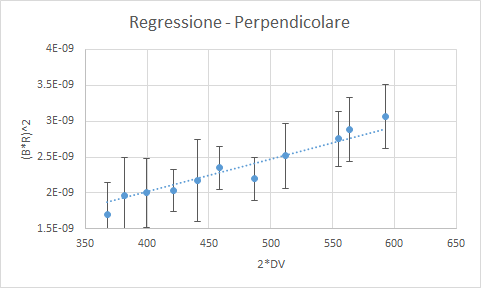
\includegraphics[scale=1.25]{retta1}			%modificare percorso
			\caption{Regressione Lineare - perpendicolare.}\label{retta1}
		\end{figure}	
		
		\begin{figure}[htpb]
			\centering
			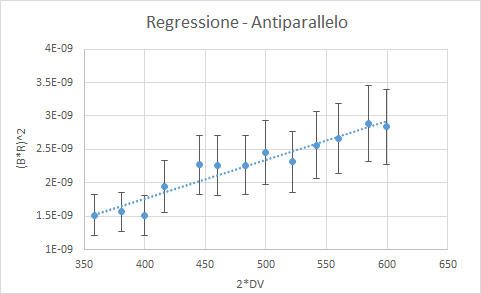
\includegraphics[scale=1.25]{retta2}			%modificare percorso
			\caption{Regressione Lineare - antiparallelo.}\label{retta1}
		\end{figure}	
		
		Con i dati ricavati da \ref{mq_perp} e \ref{mq_parall} è possibile invertire per ottenere i valori di $e/m$ calcolando l'errore tramite la derivata, in questo caso in una sola variabile. I valori ottenuti sono rispettivamente
		\begin{equation}\label{em_perp}
		e/m = \SI{1.874E+11}{\coulomb/\kilogram} \pm 1.55E+10
		\end{equation}
		e 
		\begin{equation}\label{em_perp}
		e/m = \SI{1.684E+11}{\coulomb/\kilogram}\pm 1.47E+10
		\end{equation}
		che risultano compatibili tra di loro e compatibli entrambi con il valore dichiarato di $\SI{1.7588E+11}{\coulomb/\kilogram}$.
		
		\section{Conclusioni}
		L'esperienza di verifica del rapporto $e/m$ può dirsi eseguita con successo. Entrambi i valori ottenuti, seguendo la stessa procedura ma con condizioni differenti, restituiscono infatti un valore compatibile con quello dichiarato. L'unico punto da chiarire resta la scarsa compatibilità dell'intercetta con l'origine per la seconda regressione, sebbene il limite del $95\%$ non sia poi così distante. 
	
	
\end{document}